\documentclass{beamer}

\usetheme{Berlin}
\usecolortheme{beaver}
\usepackage[backend=biber, style=numeric]{biblatex}
\usepackage{tabularx}
\newcolumntype{Y}{>{\raggedright\arraybackslash}X}


\addbibresource{biblio.bib}
\title{Digital Twins of the Heart}
\subtitle{Coursework "ROM \& Data-driven ROM" - CSMI}
\author{Rodolphe Vivant \& Antoine Ruch}
\institute{UFR of Mathematics and Informatics}
\date{\today}

\begin{document}

\begin{frame}
  \titlepage
\end{frame}

\begin{frame}{Plan}
  \tableofcontents
\end{frame}

\section{Introduction}


\begin{frame}{Context \cite{who2025cvd}}
  Cardio vascular diseases (CVD) represent the \textbf{$1^{st}$ cause of death in the world} \cite{who2025cvd} :
  \begin{itemize}
    \item \textbf{32 \%} of all global deaths in 2022
    \item \textbf{85 \%} of them were due to heart attack and stroke
    \item \textbf{38 \%} of the 18 million premature deaths (under 70) caused by CVDs
  \end{itemize}
\end{frame}

\begin{frame}{Problems \cite{gerach2021electro}}
    \begin{itemize}
        \item Direct clinical studies limited by ethical and technical constraints
        \item The complexity of the heart 
        \begin{itemize}
            \item Multi-scaled structure connected (cell $\rightarrow$ organ)
            \item Multi-physics laws intertwined (Electrical, mechanical, fluid dynamics)
        \end{itemize}
        \item Lack of predictive medicine for current treatments 
    \end{itemize}
\end{frame}

\section{Objective of a Heart's DT}
\begin{frame}{Objective}
\begin{figure}
    \centering
    \begin{minipage}{0.5\linewidth}
      \begin{itemize}
        \item Create computational models that reproduce "in silico" the physiologic structure and the multi-physics functions of a personalized heart
        \begin{itemize}
            \item \textbf{enables preventive diagnostics}
            \item \textbf{precise therapy developments and personalized planning}
        \end{itemize}
        \item The sooner and the more precise the CVD diagnostic, the more efficient the treatment
      \end{itemize}
    \end{minipage}\hfill
    \begin{minipage}{0.45\linewidth}
        \centering
        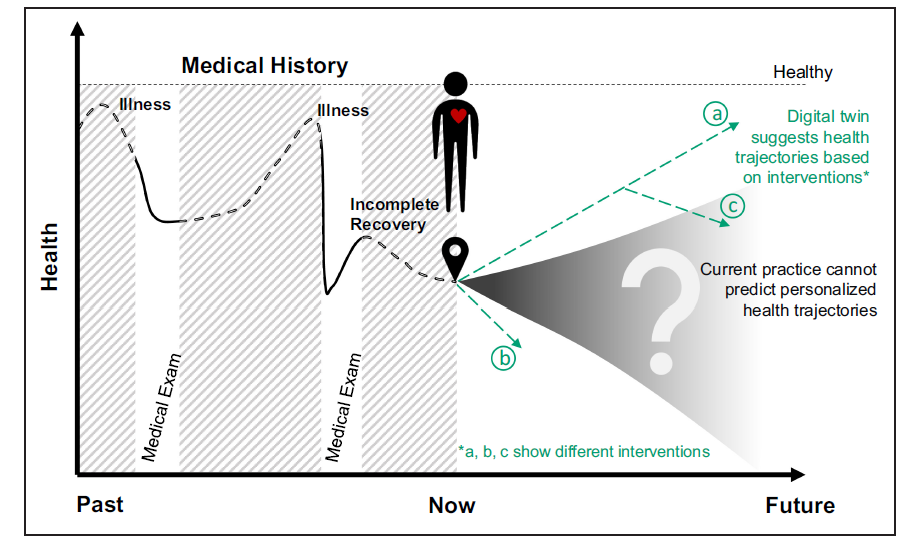
\includegraphics[width=1\linewidth]{images/DT_perso_health_trajectories.png}
        \caption{Personalized health Trajectories \cite{sel2024digital}}
        \label{fig:traject_perso}
    \end{minipage}
\end{figure}
\end{frame}

\begin{frame}{Steps of the creation of cardiovascular system models}
\begin{minipage}{0.5\linewidth}
  \centering
  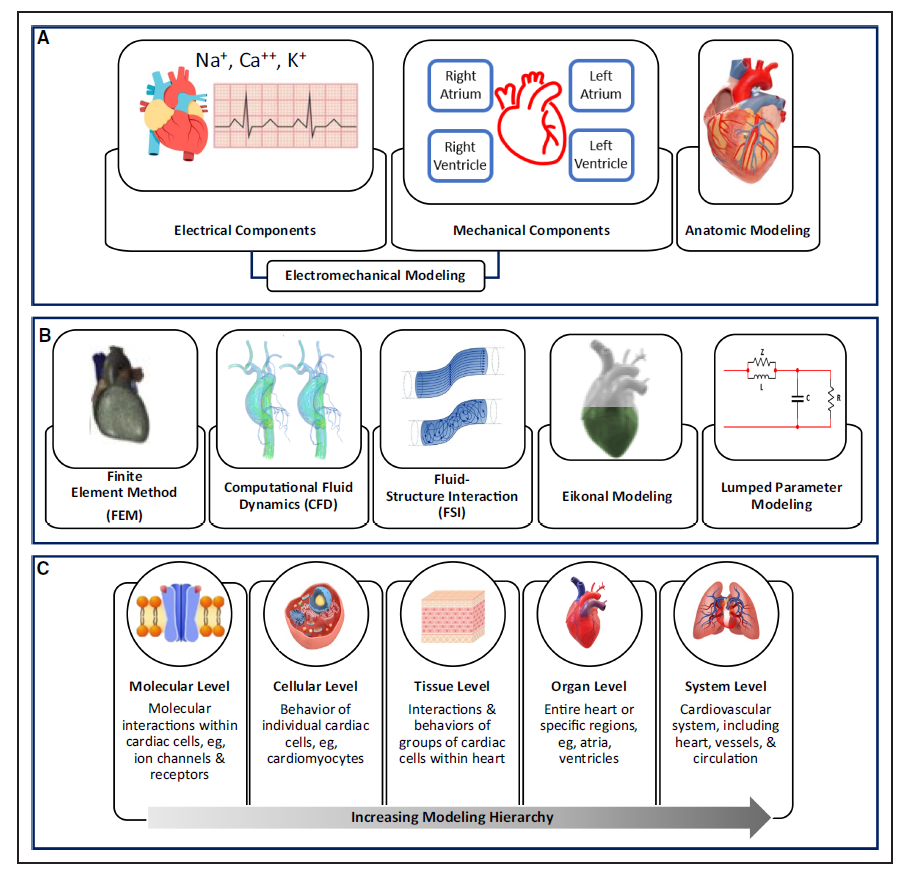
\includegraphics[width=0.95\linewidth]{images/creation_cv_system_models.png}
  \\
  \scriptsize{\textcite{sel2024digital}}
  \label{fig:step_creation_computational_model}
\end{minipage}\hfill
\begin{minipage}{0.45\linewidth}
  \begin{itemize}
    \item A : Modeling physiological aspects
    \item B : Modeling Methods
    \item C : Increasing modeling scale
  \end{itemize}
\end{minipage}
\end{frame}

\section{Architecture of a Health's DT}
\begin{frame}{Pipeline of a Health's DT}
    \begin{figure}
    \centering
    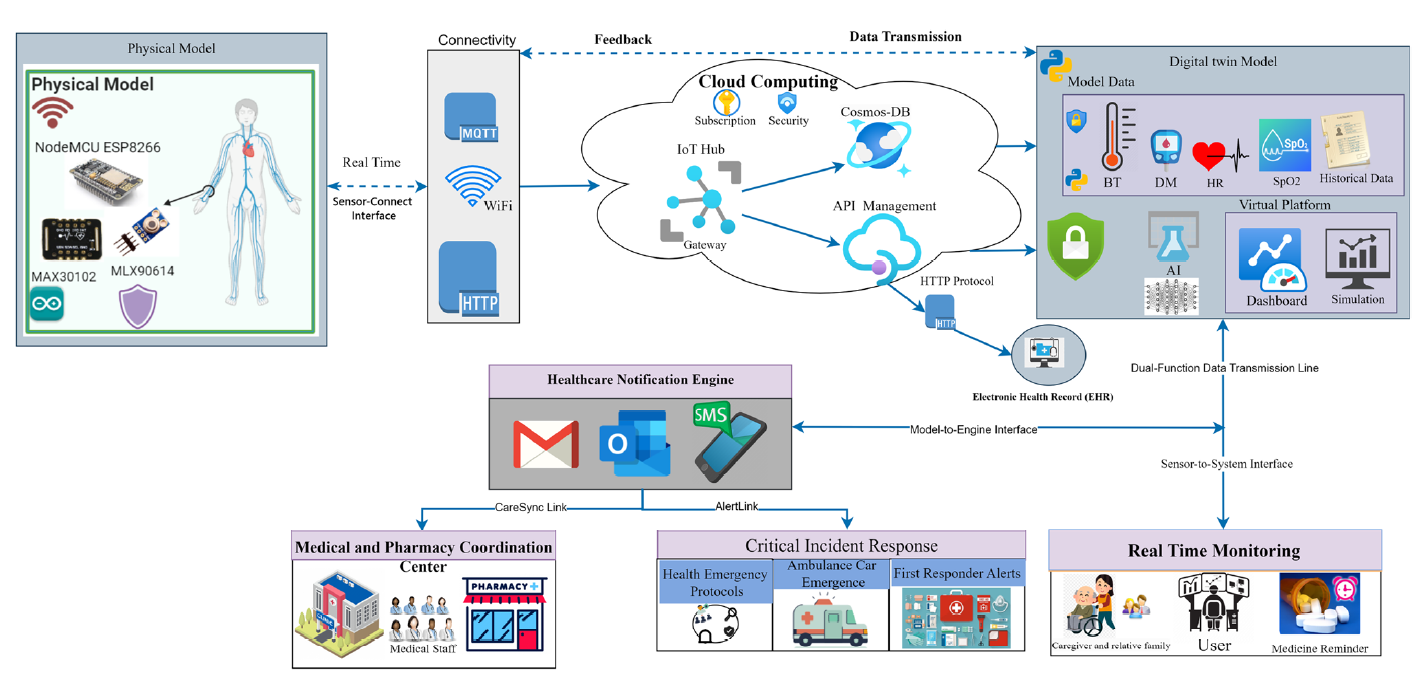
\includegraphics[width=1\linewidth]{images/Architecture_health_dt.png}
    \caption{Pipeline of health digital twin}
    \label{fig:PipelineHealthDT}
\end{figure}
\end{frame}

\section{Mathematical Models}

\subsection{Numerical Methods for Cardiac Electrophysiology}
\begin{frame}{FED (finite element discretization) for Cardiac Electrophysiology \textcite{gerach2021electro}}
  \begin{figure}
    \centering
    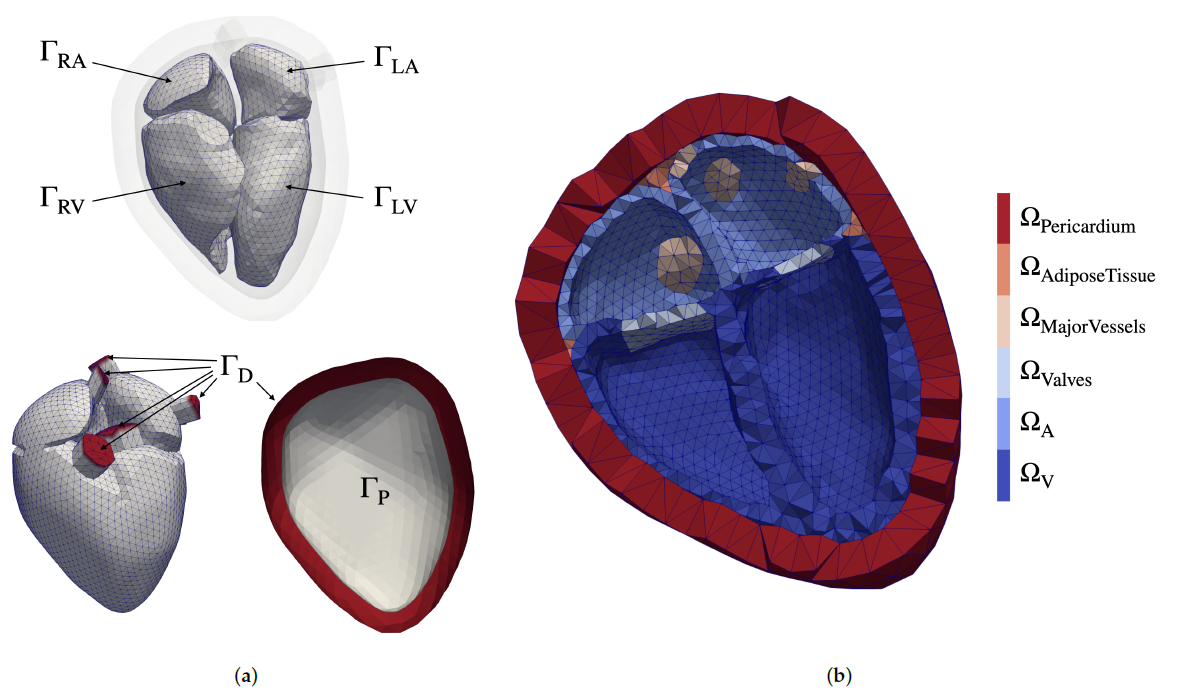
\includegraphics[width=0.8\linewidth]{images/heart_discretization.png}
    \caption{Four Chamber Heart Model discretization for FEM}
    \label{fig:heart_discretization}
\end{figure}
\end{frame}

\begin{frame}{Mathematical aspects for Cardiac Electrophysiology \cite{gerach2021electro}}
  Typical multi-physics and multi-scale model 
  \begin{itemize}
    \item \textbf{Cardiac electrophysiology (EP)} on $\Omega_{EP} = \Omega_A \cup \Omega_V \cup \Omega_{Valves}$
    \begin{itemize}
      \item On the microscopic or cellular level, reaction part
      \item The diffusion on the macroscopic level
    \end{itemize}
    \item \textbf{Cardiac mechanics (M)} to describe the deformation on $W_M = W_V \cup W_A \cup W_{Valves} \cup W_{AdiposeTissue} \cup W_{MajorVessels} \cup W_{Pericardium}$
    \item \textbf{Blood's loading conditions} imposed by the circulatory system
  \end{itemize}
  Simulation frameworks have been proposed that solve the complete \textbf{EP-M-FSI} system
\end{frame}

\begin{frame}{Solving Methods \cite{gerach2021electro}}
  \begin{itemize}
    \item In Space
      \begin{itemize}
        \item \textbf{Finite Element Method (FEM)} : in $\Omega_{M} \cup \Omega_{EP}$ to solve the coupled PDEs for the mechanical aspects
        \item with Robin Boundary conditions / Sliding contact Problem: in $\Gamma_{P}$
      \end{itemize}
    \item In Time
      \begin{itemize}
        \item \textbf{Fluid/Structure Interaction (FSI)} : in $\Omega_{M}$ for the closed loop circulatory model coupled with the FEM presented above
        \item \textbf{Operator Splitting Method} : in $\Omega_{EP}$ for the Electrophysiology equations
        \item \textbf{Space-independent ODE} : for the reaction, solved by explicit integration methods (Runge-Kutta 4, Quasi-Newton) )
      \end{itemize}
  \end{itemize}
\end{frame}

\begin{frame}{Solving Methods \cite{gerach2021electro}}
  \begin{itemize}
    \item In Time (ctd)
      \begin{itemize}
        \item \textbf{Crank-Nicolson Scheme} : for the linear PDEs modeling the diffusion
        \item \textbf{Lumped Parameters model} : Use to simplify the circulatory system modeling
      \end{itemize}
    \item \textbf{Inputs} 
      \begin{itemize}
        \item \textbf{Imagery data (MRI)} for Cardiac Anatomy, Fibers Orientation, Passive stress and Active stress
        \item \textbf{ElectroCardioGram (ECG)} data body surface potential maps (BSPM) for EP model personalization
      \end{itemize}
    \item \textbf{Outputs} :
    \begin{itemize}
      \item \textbf{Calcium Transient (CaT)} : rapid, transient increase in intracellular calcium concentration $CaT(t)=[Ca^{2+}]_i(t)$
      \item \textbf{Pressure}, \textbf{Volume} and \textbf{Flow evolution in time of left and right ventricles}
      \item ...
    \end{itemize}
  \end{itemize}
\end{frame}

\begin{frame}{Parameters and time of calculation of the experiment}
  \begin{itemize}
  \item Final discretization whith GMSH :
    \begin{itemize}
      \item For $\Omega_{M}$ : 26,681 quadratic tetrahedras (h=7.2mm, 48,780 nodes) $\rightarrow$ 135,897 DOFs
      \item For $\Omega_{EP}$ : 7,334,101 linear tetrahedras (h=0.6mm)
    \end{itemize}
  \item Run on 2019 Apple iMac (8 MPI processes)
  \item Time of calculation for 1 heartbeat (0.8s) : 20 to 24 hours of computation
  \end{itemize}
\end{frame}

\subsection{DL/ML Methods}

\begin{frame}{POD-DL-ROM \cite{Fresca2021}}
  \begin{itemize}
    \item FOM - Cardiac Electrophysiology: coupled non-linear dynamical system.
    \item \textbf{Inputs} - ionic model, conductivity... Multiple querries to build multi-scenario analysis.
    \item Proposes a POD-DL-ROM pipeline - collection of FOM snapshots for efficient ROM parameter reconstruction - enhanced with POD.
    \item \textbf{Output} - ACs, APs, ECGs... Fast and efficient evaluation.
  \end{itemize}

  \begin{figure}
      \centering
      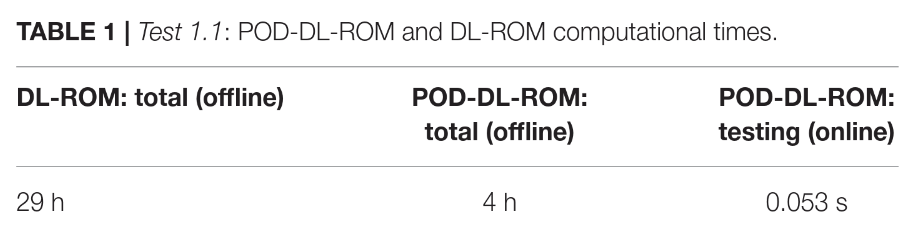
\includegraphics[width=1\linewidth]{images/POD-DL-ROM-perf.png}
      \caption{\textcite{Fresca2021}}
  \end{figure}
  
\end{frame}


\begin{frame}{Architecture}
    \begin{figure}
      \centering
      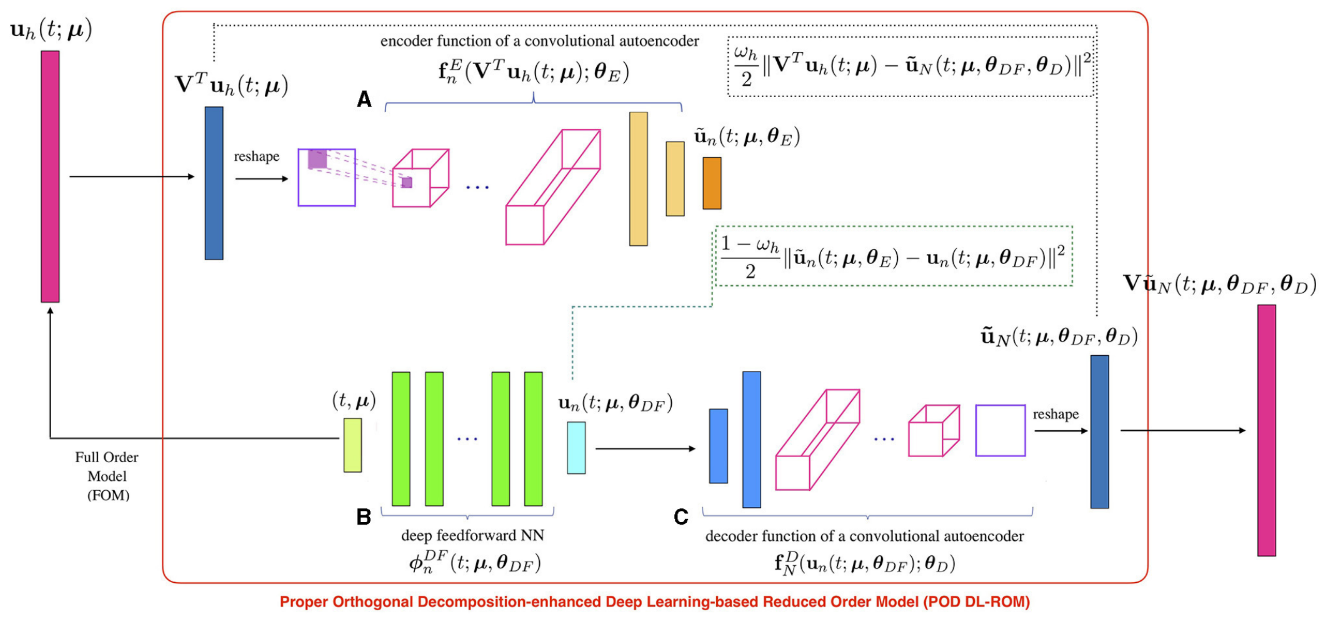
\includegraphics[width=1\linewidth]{images/POD-DL-ROM-archi.png}
      \caption{\textcite{Fresca2021}}
  \end{figure}
\end{frame}

\begin{frame}{PINNs \cite{jafari2022}}
  \begin{itemize}
    \item AI models can extract complex actionable data from time series, but require significant amounts of ground truth data. 
    \item \textbf{PINNs}: neural networks are trained to solve problems leveraging underlying physics of input data.
    \item Builds Taylor's approximations modelling the relationship between physiological features extracted from sensor measurements.
    \item Yields a Taylor approximation in the form of a PDE.
    \item The output of the network is the estimated continuous blood pressure.
  \end{itemize}
\end{frame}

\begin{frame}{Architecture}
    \begin{figure}
      \centering
      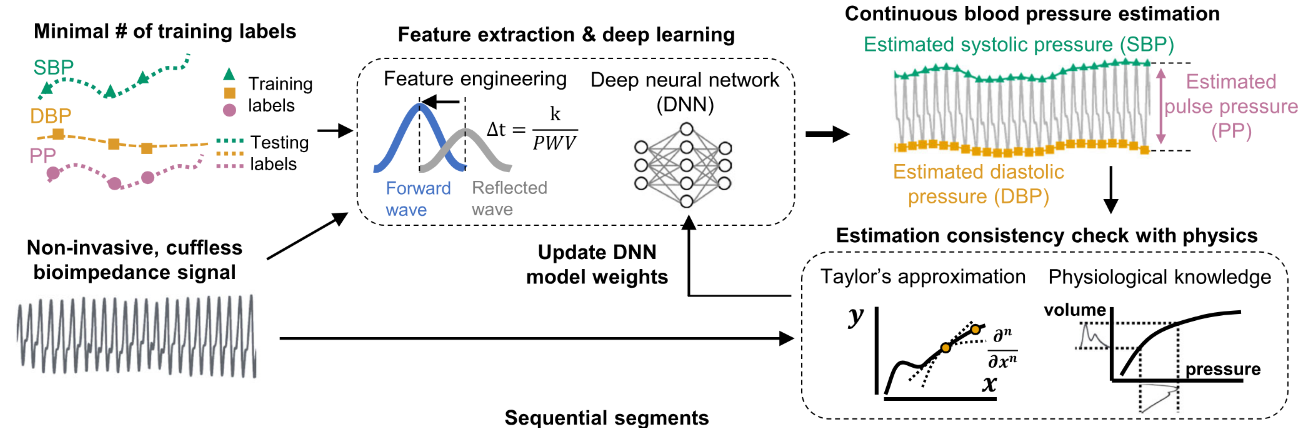
\includegraphics[width=1\linewidth]{images/PINNs-archi.png}
      \caption{\textcite{jafari2022}}
  \end{figure}
\end{frame}

\section{Clinical Data \& Continuous Monitoring}
\begin{frame}{Continuous monitoring devices}

  \scriptsize
  \begin{tabularx}{\textwidth}{|Y|c|Y|c|c|Y|c|}
  \hline
  \textbf{Device} & \textbf{Channels} & \textbf{Data} & \textbf{SPS} & \textbf{Bytes} & \textbf{Daily debit / channel} & \textbf{Paper} \\
  \hline
  Max30102 (HR/SpO2) 
  & 2 
  & HR, SpO2 
  & 512 
  & 2 
  & $512 \times 86{,}400 \times 2 \approx 88$ Mb 
  & \cite{jameil2025digital} \\
  \hline
  MLX90614 (IR thermometer) 
  & 1 
  & Body temperature 
  & 28 
  & 2 
  & $28 \times 86{,}400 \times 2 \approx 4.8$ Mb 
  & \cite{jameil2025digital} \\
  \hline
  Finapres NOVA (bio-impedance) 
  & 4 
  & BioZ1--4 
  & 112 
  & 3 
  & $112 \times 86{,}400 \times 3 \approx 260$ Mb 
  & \cite{jafari2022} \\
  \hline
  \end{tabularx}
  
\end{frame}

\section{Verification \& Validation}
\begin{frame}{Strategies \& Metrics}

    \begin{itemize}
        \item Unit tests for solvers and proposed benchmarks - still an emerging field. \textcite{Reidmen2025}
        \item Common good practices for PDE/FEM solvers: convergence studies, numerical stability (e.g. in \textcite{gerach2021electro})
        \item Compare ROM against high-fidelity snapshots - $L^2/L^\infty$ error norm fields. (e.g. in \textcite{Fresca2021})
        \item \textit{RMSE}, \textit{Bland-Altman} and \textit{Pearson’s} correlation analyses for estimated wave forms. (e.g. in \textcite{jafari2022})
        \item Classifier evaluation metrics - Accuracy, Precision, Recall, F-score. (e.g. in \textcite{burak2023})
        \item Clinical trials comparing twin-informed decisions and standard care... (WIP - \href{https://www.imperial.ac.uk/news/253154/digital-twin-heart-modelling-project-will/?utm_source}{CVD-Net})
    \end{itemize}
\end{frame}

\begin{frame}{MRSE \& Correlation analyses}
  
  \begin{figure}
      \centering
      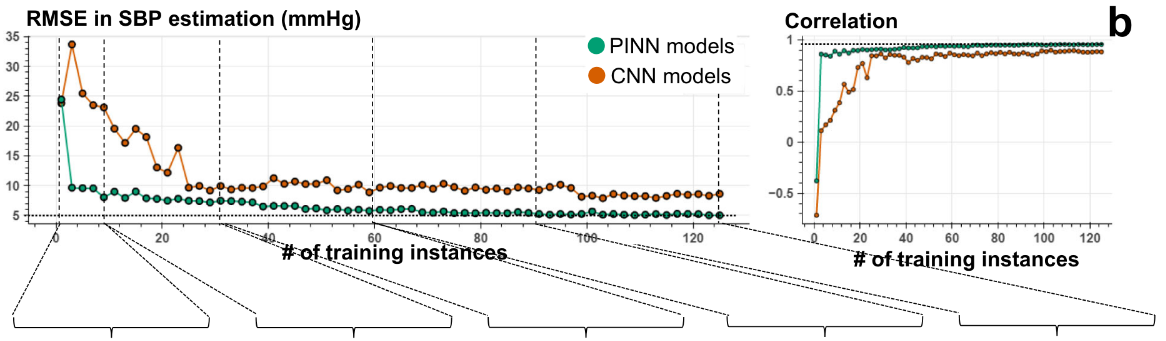
\includegraphics[width=1\linewidth]{images/MRSE.png}
      \caption{\textcite{jafari2022}}
  \end{figure}

\end{frame}

\begin{frame}{Relative error fields}
  
  \begin{figure}
      \centering
      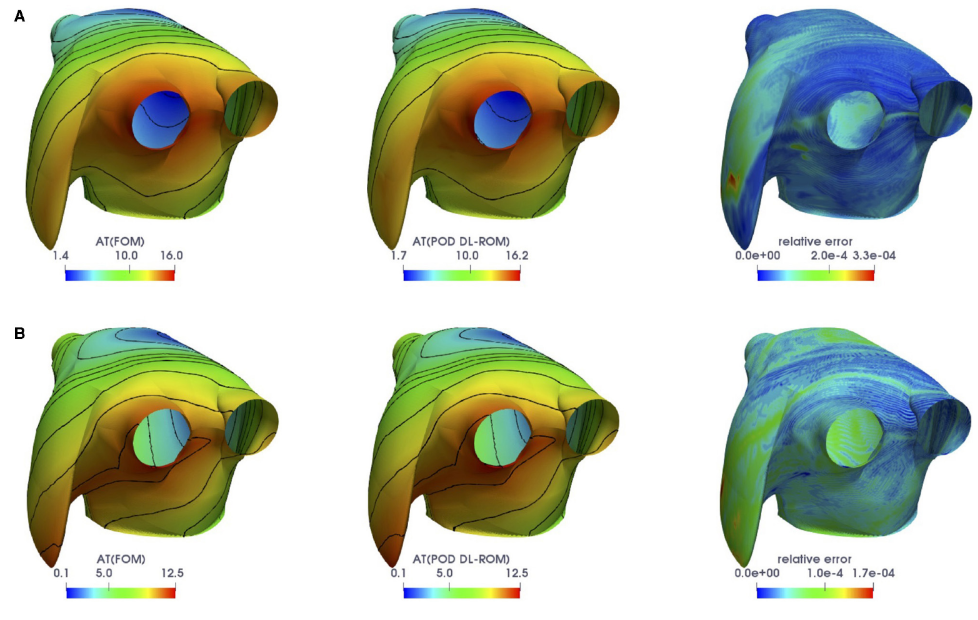
\includegraphics[width=0.7\linewidth]{images/err-fields.png}
      \caption{\textcite{Fresca2021}}
  \end{figure}

\end{frame}

\section{Deployment \& Implementation}

\begin{frame}{Deployment \& Implementation}
  \begin{itemize}
    \item IoT based DT frameworks - continuous measurements from wearable sensors and transmission through the network: bandwidths and latency.
    \item \textit{Offline}: cloud computing (e.g. MS Azure, AWS, GCC...)
    \item \textit{Online}: cloud or edge-based. Low latency crucial for monitoring.
    \item Case study: \textbf{Edge} VS \textbf{Cloud} based DT frameworks for ML classifier modules. Overall better performances of the edge framework (\textcite{burak2023}).
    \item Edge devices: cell-phones, hospital network, embedded computing (e.g. Raspberry Pi).
    \item Additional software development challenges - API for live-monitoring, CI/CD, DevOps/MLOps for maintainability and control loops based on inference metrics.
  \end{itemize}
\end{frame}

\section{Perspectives \& Limits}

\begin{frame}{Perspectives \& Limits}
  
  \textbf{Technical barriers} 
  \begin{itemize}
    \item Computational cost of current methods limits potential reach outside the private health sector. 
    \item Complexity of integrating clinical and sensor data into unified prediction models.
  \end{itemize}
  \textbf{Privacy and ethics}
  \begin{itemize}
    \item Handling of large amounts of sensitive health data. Concerns about complying to health regulations - GDPR, HIPAA... Access to open-source health data for training.
    \item Assessing the responsibility of prediction modules, control and veto mechanisms.
    \item Infrastructure security - edge based frameworks are particularly sensitive (MITM, Ransomware).
  \end{itemize}
\end{frame}

\section*{Déclaration d'assistance IA}
\begin{frame}{Déclaration d'assistance IA}
  Certaines parties de ce travail ont été préparées avec l'assistance d'outils d'Intelligence Artificielle (IA). Les outils suivants ont été utilisés (toutes les sorties vérifiées, révisées et intégrées de manière responsable par les auteurs) :
  \begin{itemize}
    \item ChatGPT (OpenAI, familles GPT-4/5) – assemblage d'une bibliographie introductive comme point de départ pour nos recherches.
  \end{itemize}
  Toutes les sorties IA ont été \textbf{vérifiées, adaptées et corrigées par les auteurs}. Les auteurs acceptent la pleine responsabilité de la justesse, de l'originalité et de l'intégrité scientifique de ce travail.
\end{frame}

\begin{frame}[allowframebreaks]{References}
    \printbibliography
\end{frame}



\end{document}
